\section{Аналитическая часть}

\subsection{Электронный документ}

Электронный документ – это документ, информация которого представ-
лена в электронной форме. Юридическая значимость такого документа может
быть получена с помощью электронной подписи, визуальное отображение подписи в документе не требуется\cite{dadaya}. Для электронного документа характерно следующее:

\begin{itemize}[label=---]
	\item аутентичность -- свойство электронного документа, гарантирующее, что электронный документ идентичен заявленному;
	
	\item достоверность -- свойство электронного документа, при котором содержание является полным и точным представлением подтверждаемых операций, деятельности или фактов и которому можно доверять в последующих операциях или в последующей деятельности;
	
	\item целостность -- состояние электронного документа, в который после его создания не вносились никакие изменения;
	
	\item пригодность для использования -- свойство электронного документа, позволяющее его локализовать и воспроизвести в любой момент времени.
\end{itemize}

\subsection{Постановка задачи}

Объём административных процедур, требующих документального подтверждения, ежегодно увеличивается примерно на 15\%\cite{dadaya}. Бумажный документооборот обладает следующими критическими проблемами:
 
\begin{itemize}[label=---]
	\item практически для каждой административной процедуры имеется несколько шаблонов документов, что в дальнейшем затрудняет классификацию, хранение и поиск необходимого документа;
	
	\item в зависимости от типа документа срок его хранения может составлять от нескольких минут до 75 лет\cite{dadaya}. В то время как документооборот постоянно увеличивается, стоимость организации и ведения архива увеличивается примерно на 30\% ежегодно. Процедуры поиска и классификации документа могут занимать от нескольких часов до нескольких дней;
	
	\item важным аспектом является защита конфиденциальных данных, поскольку физические архивы более подвержены риску компрометации критической информации и персональных данных из-за человеческого фактора;
	
	\item в зависимости от количества контрагентов, необходимых для проведения процедуры, и их территориального расположения время, затрачиваемое на оформление процессов бумажного документооборота, может быть существенно увеличено. Ежегодная доля документов, в которых участвуют межрегиональные или межгосударственные ведомства, составляет 25\%. Наглядный пример такого бизнес-процесса представлен на рис. \ref{fig:sign-flow}. Отказ одного из контрагентов имеет решающее значение при межгосударственном бумажном оформлении, поскольку перезапускает весь процесс.
\end{itemize}

\begin{figure}[h!btp]
	\centering
	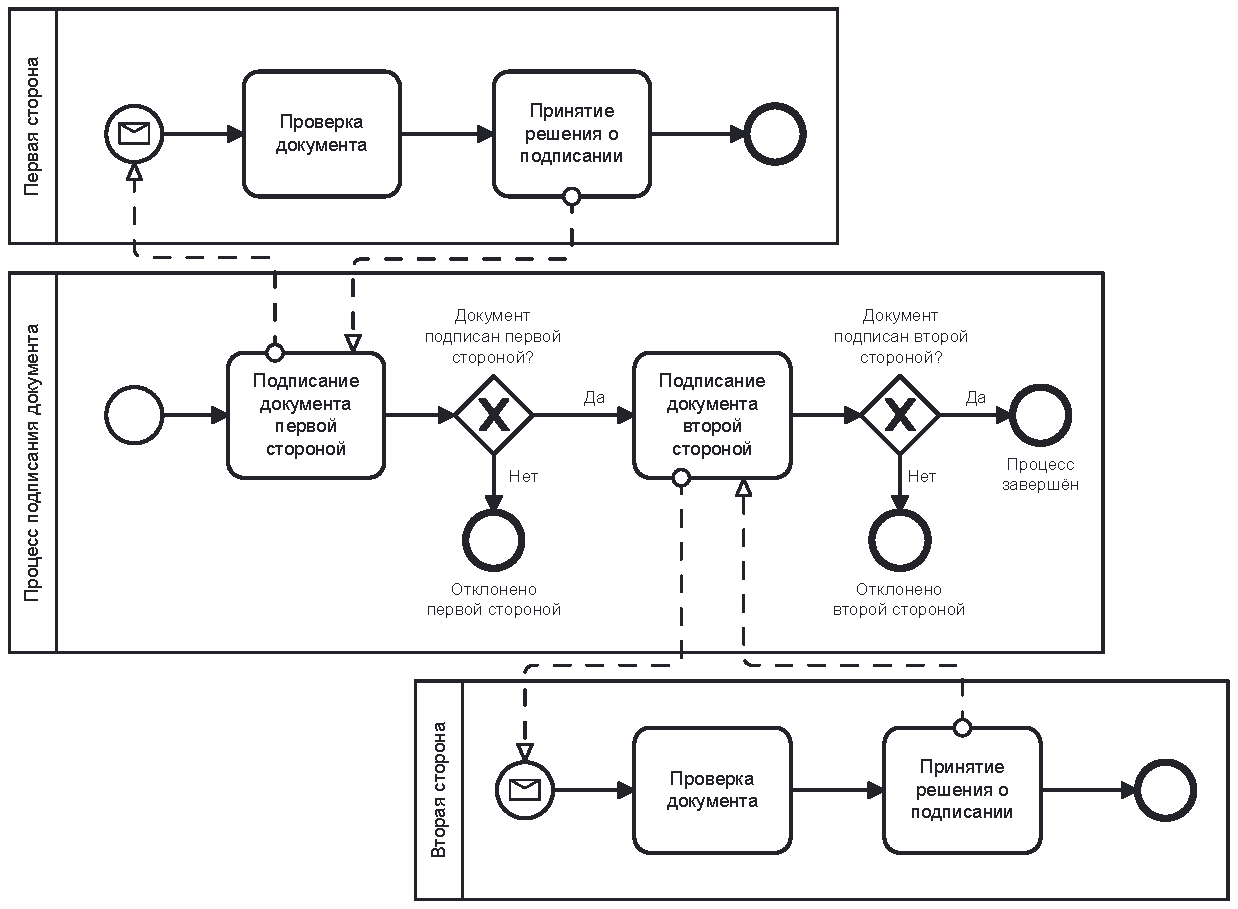
\includegraphics[width=0.9\textwidth]{inc/sign_flow_bpmn.pdf}
	\caption{Модель бизнесс-процесса подписания документа}
	\label{fig:sign-flow}
\end{figure}

Данные недостатки приводят к развитию сферы цифрового документооборота\cite{dadaya}, как одной из основных приоритетных задач цифровизации государственного и частного сектора. 

Для обработки большого объёма операций с электронными документами между многочисленными, в том числе межгосударственными контрагентами, были разработаны системы электронного документооборота (СЭД). СЭД должна соответствовать современным стандартам безопасности, эффективности и надёжности\cite{dadaya}, где ключевым требованием является своевременное выполнение процессов и отказоустойчивость системы. Современные СЭД ориентированы на управление процессами, а не на управление потоками данных\cite{dadaya}, поскольку абстрактная структура документа практически не влияет ни на одну из критических функций\cite{dadaya}, но переходы состояний и их порядок сильно влияют на каждый аспект такой системы. 

С точки зрения управления цифровыми документами, управление временем включает в себя следующее: планирование рабочего процесса, оценку продолжительности выполнения, выполнения процесса при соблюдении всех заданных временных ограничений\cite{reward2}. Поэтому моделирование таких рабочих процессов документооборота с ограничениями по времени для поиска оптимального обхода состояний является сложной задачей\cite{dadaya}.

\subsection{Моделирование с помощью сетей Петри}

Сеть Петри представляет собой модель двудольного графа\cite{dadaya}, состоящую из двух классов узлов, мест и переходов. Места соединяются переходами с помощью дуг и могут содержать фишки, маркировка (текущее состояние) задаётся количеством фишек. 

Переходы -- это действия, которые могут происходить при изменении состояния системы и могут срабатывать только в том случае, если они включены (должны быть выполнены все предварительные условия). Когда переход срабатывает, он переносит токены из своих входных мест в свои выходные места. Количество передаваемых токенов зависит от мощности каждой дуги. Математически сеть Петри определяется как кортеж:

\begin{equation}\label{eq:petri}
	N = (P, T, I, O, M_0),
\end{equation}

где $P = \{p_1, p_2, ..., p_m\}$ множество мест, $T = \{t_1, t_2, ..., t_n \}$ множество переходов, $I \subset P \times T$ множество входящих дуг, $O \subset T \times P$ множество исходящих дуг, $M_0 = (m_{01}, m_{02}, …, m_{0m})$ начальная разметка.

\subsubsection{Описание поведения системы}

В качестве математического инструмента сеть Петри можно использовать для создания различных алгебраических уравнений и математических моделей, описывающих поведение системы.

Рассмотрим четыре наиболее распространённых поведения системы\cite{dadaya}:

\begin{enumerate}
	\item последовательное выполнение;
	
	\item параллельное выполнение;
	
	\item конкуренция;
	
	\item синхронизация.
\end{enumerate}

Последовательное выполнение в терминах сетей Петри можно смоделировать, как показано на рисунке \ref{fig:sequential}. Каждый переход срабатывает один за другим.

\begin{figure}[h!btp]
	\centering
	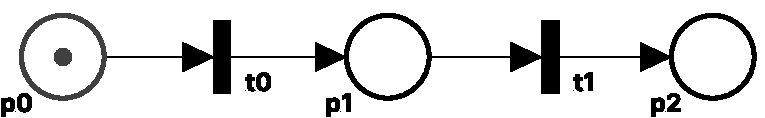
\includegraphics[width=0.9\textwidth]{inc/sequential.pdf}
	\caption{Модель последовательного выполнения}
	\label{fig:sequential}
\end{figure}

Параллельное выполнение можно смоделировать, как показано на рисунке \ref{fig:concurrent}. Имеется три параллельных перехода, каждый из которых после получения фишки включается и может сработать.

\begin{figure}[h!btp]
	\centering
	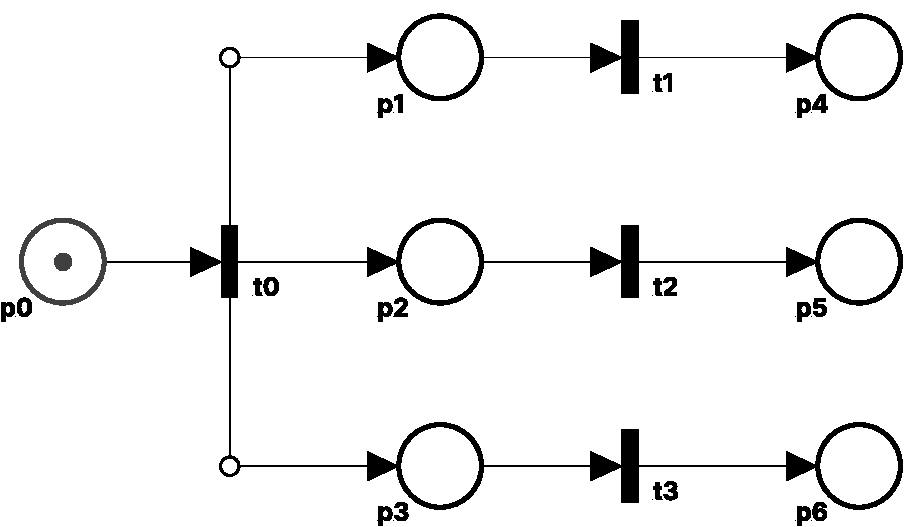
\includegraphics[width=0.9\textwidth]{inc/concurrent.pdf}
	\caption{Модель параллельного выполнения}
	\label{fig:concurrent}
\end{figure}

\clearpage

Конкурентное поведение, также известное как принятие решений, можно смоделировать, как показано на рис. \ref{fig:competetive}. Все три перехода активны и могут сработать, но сработает только один, оставив два других перехода в отключённом состоянии. Если переход связан со временем срабатывания, будет выбран переход с минимальным временем, необходимым для срабатывания.

\begin{figure}[h!btp]
	\centering
	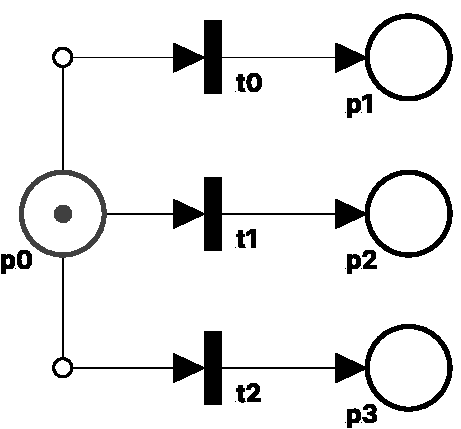
\includegraphics[width=0.6\textwidth]{inc/competetive.pdf}
	\caption{Модель конкурентного поведения}
	\label{fig:competetive}
\end{figure}

Синхронизацию можно смоделировать как показано на рис. \ref{fig:sync}, последний переход $t_2$ будет активирован только в том случае, если в соединённых позициях $p_2$ и $p_3$ есть фишки.

\begin{figure}[h!btp]
	\centering
	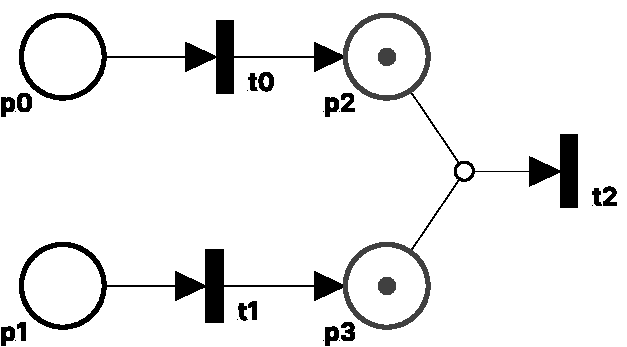
\includegraphics[width=0.6\textwidth]{inc/sync.pdf}
	\caption{Модель синхронизации системы}
	\label{fig:sync}
\end{figure}

\subsubsection{Раскрашенная сеть Петри}

Раскрашенная сеть Петри -- это кортеж, состоящий из восьми элементов:

\begin{equation}
	CPN = <P, I, T, G, A, E, Z, C>.
\end{equation}

1. $P$ -- конечное множество позиций. С каждой позицией может
быть связана определённая маркировка, которая учитывает наличие
в данной позиции различных типов ресурсов. Маркировка позиции
$p \in P$ представляет собой мультимножество, например, следующего
вида: $m(p) = (1'r,2'b,1'g)$. Здесь $r, b, g$ -- переменные указанных цветовых типов, определяющие различные виды ресурсов, а цифры, стоящие перед апострофами, -- количество фишек соответствующего типа
в позиции $p \in P$.

2. $I(p)$ -- функция инициализации сети \texttt{CPN}.

3. $Т$ -- конечное множество переходов.

4. $G$ -- блокировочная функция, описывающая дополнительные условия, которые должны быть выполнены для срабатывания перехода $t \in T$.

5. $A$ -- конечное множество ветвей, связывающих между собой позиции и переходы.

6. $E(a)$ -- функция, задающая выражения на ветвях $a \in A$.

7. $Z$ -- конечное множество непустых типов, называемое цветами.

8. $C(p)$ -- цветовая функция, определяющая множество типов цветов, разрешённых для каждой позиции.

\subsubsection{Раскрашенная сеть Петри с временным механизмом}

Существует ряд задач моделирования, в которых необходимо учитывать не только последовательность событий, но и время их наступления, а также продолжительность. Для этой цели предусмотрено расширение возможностей раскрашенных сетей Петри путём введения временного механизма -- \texttt{Timed CPN (tCPN)}:

\begin{equation}
	tCPN = <P, I, T, G, A, E, Z, C, \tau, \varDelta t>.
\end{equation}

В модель системы вводятся часы, показывающие глобальное время $\tau$.

\subsubsection{Стохастические сети Петри}

Стохастическая временная сеть Петри -- \texttt{Stochastic Timed CPN (sTPN)} расширена за счёт переходов по времени срабатывания\cite{introspn}, как детерминированных, так и стохастических\cite{dadaya}. Этот тип сетей широко используется\cite{introspn2}, так как большинство реальных процессов лучше описываются вероятностными моделями. Математически \texttt{sTPN} определена как кортеж:

\begin{equation}
	sTPN = (P, T, I, O, M_0, \Lambda).
\end{equation}

1. $(P, T, I, O, M_0)$ сеть Петри (\ref{eq:petri}).

2. $\Lambda = (\lambda_1, \lambda_2, ..., \lambda_3)$, где $\lambda_i$ случайное распределение времени срабатывания перехода.

Случайное распределение времени можно обозначить[8] как вероятность времени срабатывания:

\begin{equation}
	\lambda_i(x) = P\{t_i < x\}.
\end{equation}

Переходы с нулевым временем срабатывания называются немедленными переходами и подходят, когда продолжительность события можно игнорировать. Запуск перехода представляет собой атомарную операцию: токены удаляются из его входных мест и помещаются в его выходные места с помощью одной неделимой операции, в отличие от синхронизированных по времени моделей сетей Петри, где переходы разбиваются на три фазы.  

Задержка срабатывания связана с каждым переходом и определяет количество времени, которое должно пройти, прежде чем переход сможет сработать. Эта задержка срабатывания является случайной величиной с отрицательной экспоненциальной функцией плотности вероятности (\texttt{PDF}). Параметром \texttt{PDF}, связанным с переходом $t_i$, является скорость перехода $\lambda_i (M_j)$, которая может зависеть от маркировки. Средняя задержка перехода $t_i$ при маркировке $M_j$ равен:  

\begin{equation}
	[\lambda_i(M_j)]^{-1}.
\end{equation}

Всякий раз, когда изменение маркировки включает переход, который ранее не был включён с момента его последнего срабатывания, этот переход выбирает экземпляр задержки срабатывания из связанного отрицательного экспоненциального распределения \texttt{PDF} и устанавливает таймер на значение экземпляра выборочной задержки. Пока переход включён, таймер уменьшается с постоянной скоростью. Если переход отключён из-за срабатывания конфликтующего перехода, таймер останавливается и декремент возобновляется, когда переход снова включается. Когда таймер достигает нулевого значения, срабатывает переход.

\subsubsection{Анализ стохастической сети Петри}
Рассмотрим два основных метода анализа моделей \texttt{sTPN}:

\begin{enumerate}
	\item прямой переходный анализ;
	
	\item обратный переходный анализ.
\end{enumerate}

Прямой переходный анализ\cite{transient} оценивает дерево, состоящее из мест, где дуги соединены с переходами и вероятностями их срабатывания. Места — это классы стохастических состояний\cite{dadaya}, включающие маркировку, функцию плотности вероятности (\texttt{PDF}) таймеров и матрицу их границ различий (\texttt{DBM}). Для заданного времени $T$, перечисление продолжается до тех пор, пока дерево не покроет переходные срабатывания \texttt{sTPN} к моменту времени $T$ с вероятностью большей, чем $1-\epsilon$, где $\epsilon > 0$ это ошибка.

Обратный переходный анализ, в то время как стандартный анализ переходных процессов перечисляет одно очень большое дерево событий, регенеративный анализ избегает перечисления повторяющихся поддеревьев, основанных на одной и той же точке регенерации (где все общие таймеры сбрасываются или включаются на детерминированное время). Шаг по времени используется для выбора равноотстоящих точек времени, в которых оцениваются переходные вероятности (непосредственно или путём решения уравнений восстановления Маркова).

\subsection{Квантовое моделирование}

Квантовые явления остаются малоизученными и непонятными для большинства людей, в основном потому, что квантовая механика явно не проявляется на уровне обыденного опыта. Доступ к пониманию механизмов квантовых систем часто требует специализированных лабораторий и математических знаний, которые не являются частью общего образования. Однако для интуитивного понимания квантовой механики глубокие математические знания могут быть необязательны. С развитием квантовых компьютеров возникает вопрос о возможности их использования для квантовых игр\cite{quantum-games}, которые могут стать полезным инструментом для демонстрации квантовых явлений\cite{quantum-theory}. Такие игры могут быть адаптированы для демонстрации различных аспектов квантового поведения, что особенно важно при ограниченных ресурсах. Алгоритмы искусственного интеллекта, разработанные для этих игр, могут использовать возможности квантовых вычислений для анализа ходов\cite{quantum-discrete}. Развитие таких алгоритмов может привести к улучшению квантовых технологий\cite{quantum-discrete2}.

\subsubsection{Фазовое пространство}

Фазовое пространство (ФП) в классической механике и статистической физике\cite{ps}, многомерное пространство всех обобщённых координат $q_1$ и обобщённых импульсов $p_i, i = 1, 2,..., N$, механической системы с $N$ степенями свободы. ФП имеет размерность $2N$ и может быть описано с помощью ортогональной системы координат с $2N$ осями соответственно числу обобщённых координат и импульсов. Состояние системы изображается точкой с координатами $q_i, p_i,..., q_N, pn$, а изменение состояния системы во времени -- движением точки вдоль линии, называемой фазовой траекторией. Для ФП можно ввести понятие фазового объёма и понятия геометрии для множественных измерений. Фазовое пространство -- основное для классической статистической механики, изучающей функции распределения системы многих частиц\cite{quantum-discrete3}. Методы ФП успешно применяются также в теории нелинейных колебаний. Пример отображения двумерного фазового пространства представлен на рисунке \ref{fig:phase2d}.

\begin{figure}[h!btp]
	\centering
	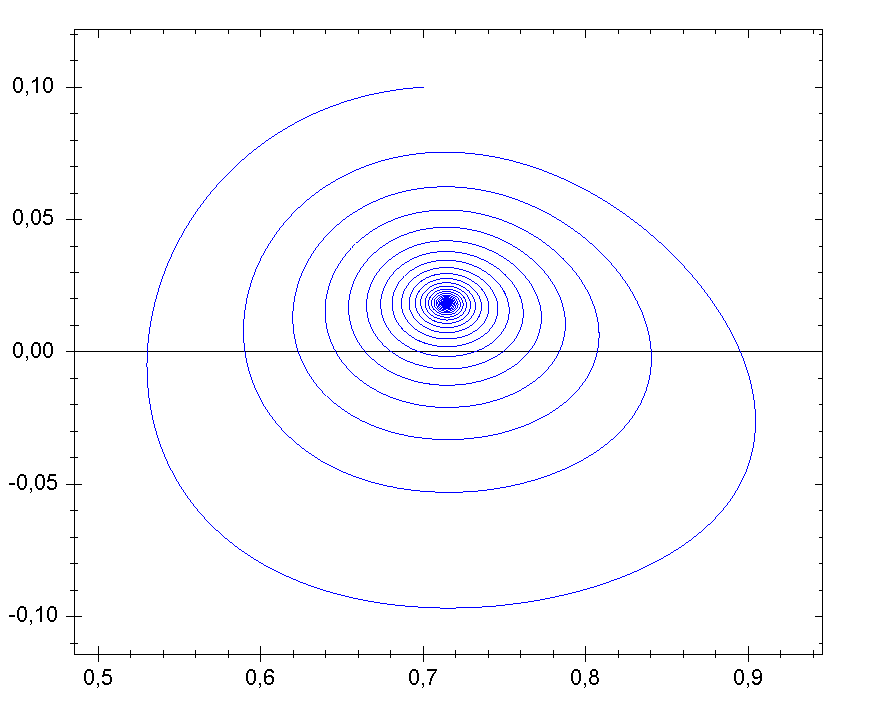
\includegraphics[width=0.75\textwidth]{inc/phase2d.png}
	\caption{Двумерное фазовое пространство}
	\label{fig:phase2d}
\end{figure}

\subsubsection{Квантовые шахматы}

Квантовые шахматы расширяют классический вариант использованием фазового пространства и принципа суперпозиции. Пример реализации партии квантовых шахмат\cite{5dchess} представлен на рисунке \ref{fig:chess}.

\begin{figure}[h!btp]
	\centering
	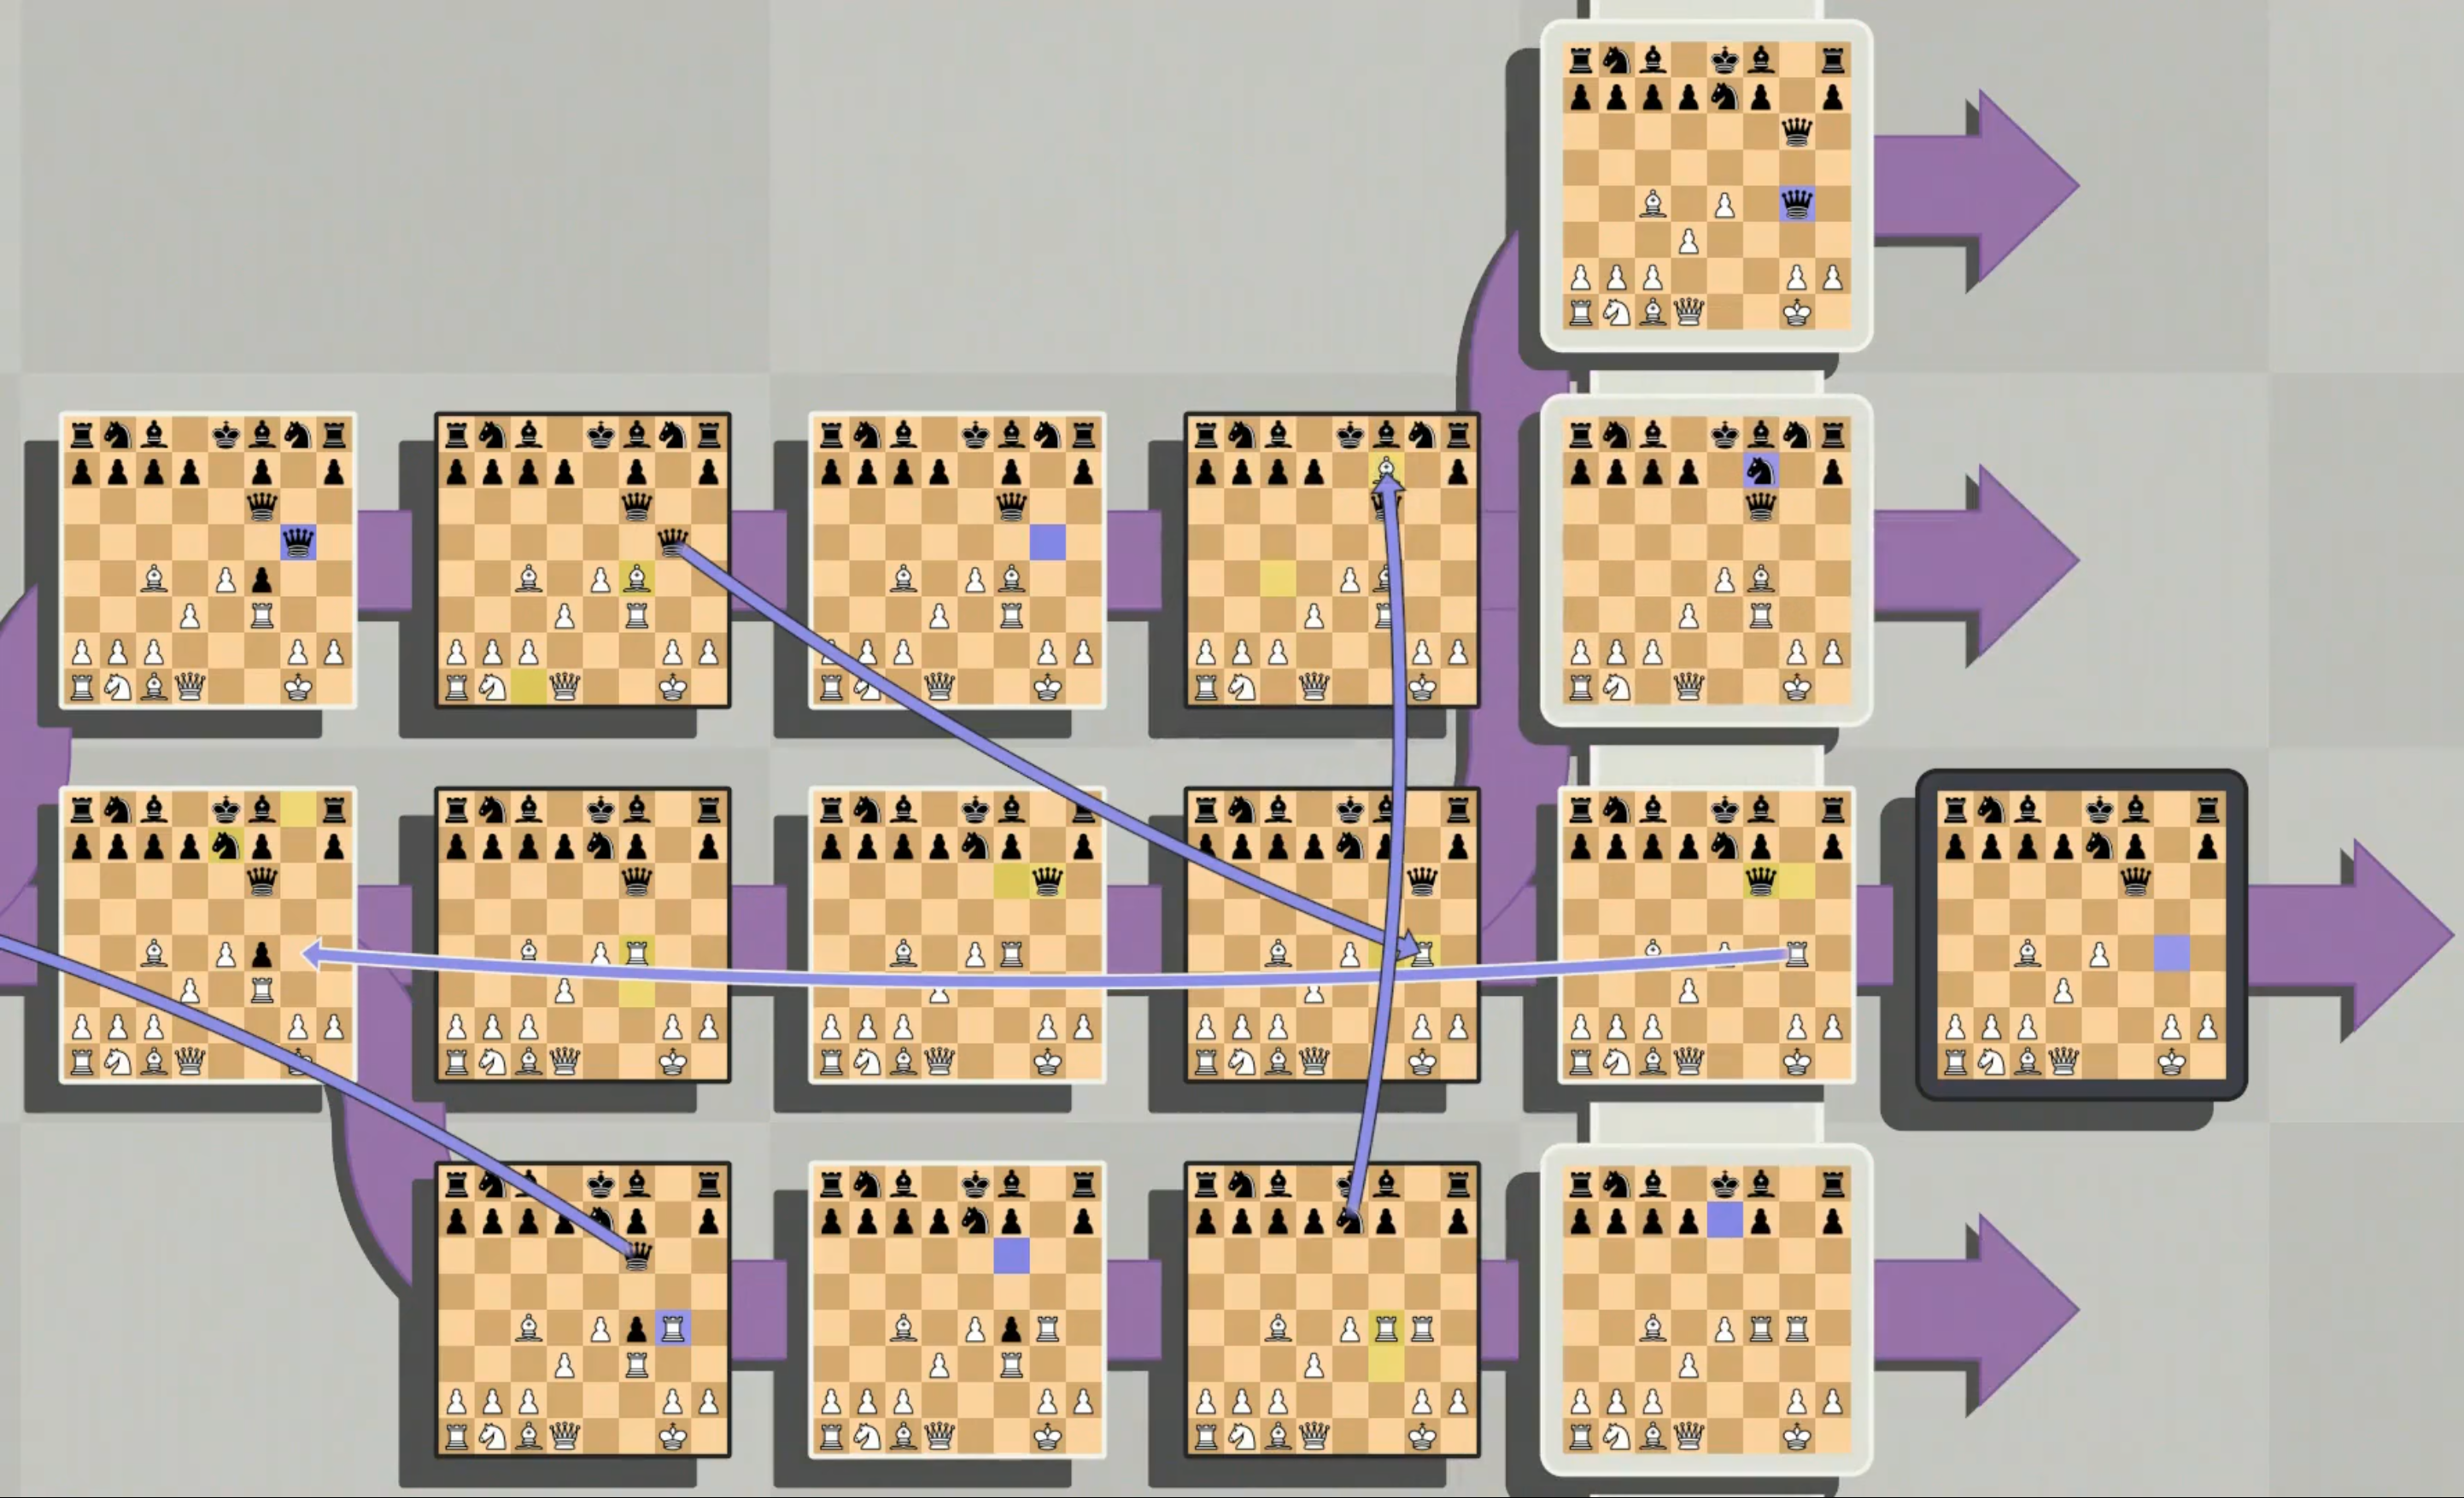
\includegraphics[width=0.75\textwidth]{inc/chess.png}
	\caption{Игровое поле}
	\label{fig:chess}
\end{figure}

Классические шахматы имеют устоявшиеся алгебраические \\* обозначения\cite{fide}, для квантовых шахмат справедливо следующее:

\begin{itemize}[label=---]
	\item неквантовое перемещение: (\textit{источник})(\textit{цель});
	\item квантовое разделение: (\textit{источник})$\wedge$(\textit{цель1})(\textit{цель2});
	\item квантовое слияние: (\textit{источник1})(\textit{источник2})$\wedge$(\textit{цель});
	\item превращение пешки: (\textit{источник})(\textit{цель})(\textit{фигура})
\end{itemize}

Все неквантовые ходы включают в себя один источник и одну цель, рокировка тоже может полностью быть описана как источником король и цель короля. Добавление дополнительных символов в строку хода для получения более подробного описания, как это принято в стандартных шахматах, является сложной задачей, учитывая природу суперпозиции. Ещё одно соображение заключается в том, что в квантовых шахматах используются измерения. Расширенная нотация с учётом измерения выглядит как: (\textit{ход}).(\textit{измерение}). Тип измерения определяется по типу хода, который соответствует строке хода, действующей на текущее состояние игры.

Для описания состояния доски используется гибридное классическое квантовое представление состояний размером 64 кубита, где 0 это <<свободное>> состояние, а 1 -- <<занятое>>:

\begin{equation}
	|\psi_\beta\rangle = \sum\limits_{i}A_i|q_o^{(i)},...q_{63}^{(i)}\rangle, q_j\in\{0, 1\}.
\end{equation}

Это представление состояния похоже на представление <<бит-доски>>, используемое в классических шахматах\cite{fide}, где наше состояние аналогично суперпозиции <<бит-доски>> <<все фигуры>>. Поверх этой суперпозиции занятости храниться классическая информация о типе для каждого квадрата. Эта информация состоит из одного вектора размерностью в 64 элемента, который описывает, какая фигура (если таковая имеется) занимает данную клетку.

\begin{equation}
	\vec{v} = \{v_0,...v_{63}\},v_i\in\{0, P, N, B, R, Q, K, p, n, b, r, q, k\}.
\end{equation}

Значения $v_i$ соответствуют стандартным значениям $FEN$ для шахматных фигур\cite{fen}: строчные буквы обозначают чёрные фигуры, белые фигуры -- заглавные, а 0 -- пустой. Клетка занята, или частично занята фигурой, если существует ненулевая вероятность найти эту фигуру в этом квадрате.

Для каждого хода можно посчитать его вероятность:

\begin{equation}\label{eq:chessprob}
	P_m(\vec{v},F)=\bigwedge\limits_{i} C_i(m,\vec{v}, F).
\end{equation}

где $C_{m,i}(\vec{v} , F)$ -- множество ограничений описывающих текущее состояние для возможности совершения хода $m$.

\subsubsection{Стандартный ход}

Стандартный ход (англ. \texttt{Standard Slide} (\texttt{SS})) -- это эквивалент стандартного шахматного хода для слонов, ладей и ферзей в квантовых шахматах. Эти фигуры перемещаются по траектории, поэтому необходимо учитывать занятость клеток между источником и целью, для этого необходима вспомогательная переменная, отражающая <<путь>>. Уравнение возможности стандартного перехода имеет следующий вид:

\begin{equation}\label{eq:chessstandard}
	P_{SS} = (v_s \in \{B,R,Q\}) \wedge valid(t,s,v_s) \wedge ((v_t = 0) \vee (v_t = v_s)).
\end{equation}

где $valid$ -- процедура проверки возможности хода, исходя из формулы вероятности хода.

\subsubsection{Второй шаг при суперпозиции} 

В стандартных шахматах разрешён шаг второй пешки при первом ходе любой пешки. Если путь не заблокирован, пешка может продвинуться на две клетки вперёд. Уравнение возможности такого хода при наличии суперпозиции:

\begin{equation}
	P_{PTS} = (v_s = P) \wedge (v_t \neq 0) \wedge (v_t \neq P) \wedge two\_step(t,s).
\end{equation}

Пример хода показан на рисунке \ref{fig:twostep}.

\begin{figure}[h!btp]
	\centering
	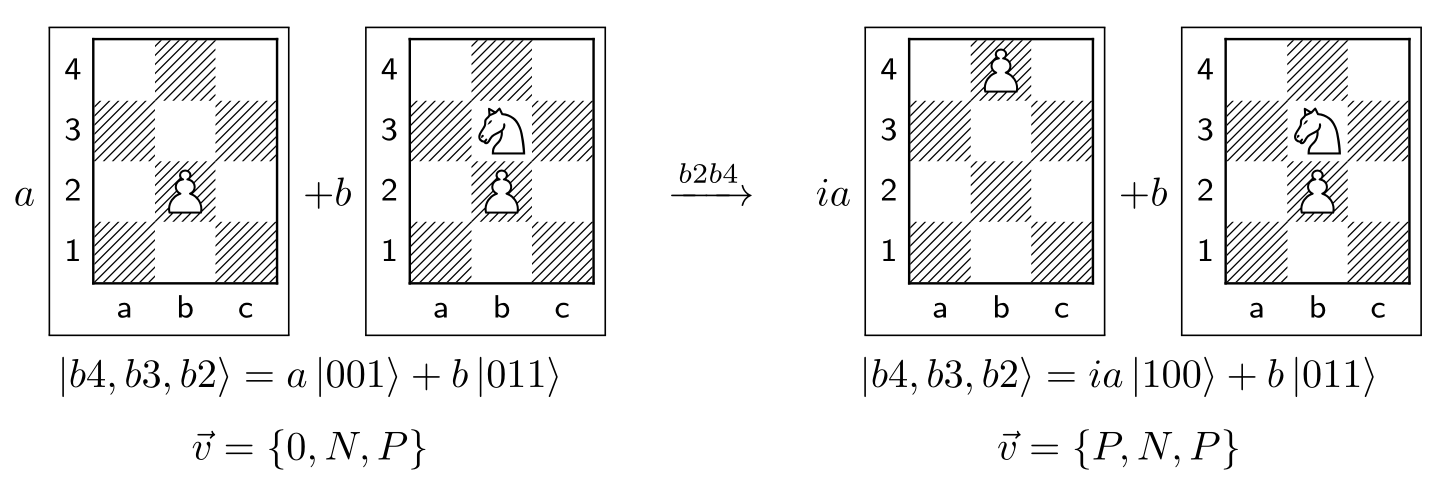
\includegraphics[width=1\textwidth]{inc/twostep.png}
	\caption{{Ход пешки с учётом суперпозиции}}
	\label{fig:twostep}
\end{figure}

\subsubsection{Вывод}

Используя метод квантовых шахмат можно просчитать вероятность нахождения документа в каждом состоянии, по принципу суперпозиции документ одновременно находится во всех состояниях сразу и ни в одном. По аналогии с шахматами может быть получен путь документа.

\clearpage

